\documentclass[a4paper, 10pt, ]{article}

\usepackage[slovak]{babel}

\usepackage[utf8]{inputenc}
\usepackage[T1]{fontenc}

\usepackage[left=4cm,
			right=4cm,
			top=2.1cm,
			bottom=2.6cm,
			footskip=7.5mm,
			twoside,
			marginparwidth=3.5cm,
			%showframe,
			]{geometry}

\usepackage{graphicx}
\usepackage{xcolor}

% ------------------------------

\usepackage{lmodern}

\usepackage[tt={oldstyle=false,proportional=true,monowidth}]{cfr-lm}

% ------------------------------

\usepackage{amsmath}
\usepackage{amssymb}
\usepackage{amsthm}

\usepackage{booktabs}
\usepackage{multirow}
\usepackage{array}
\usepackage{dcolumn}

\usepackage{natbib}

\usepackage[singlelinecheck=true]{subfig}


% ------------------------------


\usepackage{sectsty}
\allsectionsfont{\sffamily}


\usepackage{titlesec}
\titleformat{\paragraph}[hang]{\sffamily  \bfseries}{}{0pt}{}
\titlespacing*{\paragraph}{0mm}{3mm}{1mm}


\usepackage{fancyhdr}
\fancypagestyle{plain}{%
\fancyhf{} % clear all header and footer fields
\fancyfoot[C]{\sffamily {\bfseries \thepage}\ | {\scriptsize\oznacenieCasti}}
\renewcommand{\headrulewidth}{0pt}
\renewcommand{\footrulewidth}{0pt}}
\pagestyle{plain}


% ------------------------------


\makeatletter

	\def\@seccntformat#1{\protect\makebox[0pt][r]{\csname the#1\endcsname\hspace{5mm}}}

	\def\cleardoublepage{\clearpage\if@twoside \ifodd\c@page\else
	\hbox{}
	\vspace*{\fill}
	\begin{center}
	\phantom{}
	\end{center}
	\vspace{\fill}
	\thispagestyle{empty}
	\newpage
	\if@twocolumn\hbox{}\newpage\fi\fi\fi}

	\newcommand\figcaption{\def\@captype{figure}\caption}
	\newcommand\tabcaption{\def\@captype{table}\caption}

\makeatother


% ------------------------------


\def\naT{\mathsf{T}}

\hyphenpenalty=6000
\tolerance=6000


% ------------------------------


\usepackage[pdfauthor={MT},
			pdftitle={AR},
			pdfsubject={},
			pdfkeywords={},
			linkbordercolor = white,
			%citebordercolor = white,
			breaklinks,
			]{hyperref}


\def\oznacenieCasti{AR07 - LS2019}





\begin{document}





\fontsize{12pt}{22pt}\selectfont

\centerline{\textsf{Adaptívne riadenie} \hfill \textsf{\oznacenieCasti}}

\fontsize{18pt}{22pt}\selectfont





\begin{flushleft}
    \textbf{\textsf{Model Reference Control vo všeobecnosti}}
\end{flushleft}





\normalsize

\bigskip

\tableofcontents

\bigskip

\vspace{18pt}






\noindent
V predchádzajúcich častiach sme uvažovali riadený systém, ktorého stavové veličiny sú merateľné a navyše matica $A$~má Frobeniovu kanonickú formu. To umožnilo použiť zákon riadenia v~tvare stavového regulátora.

Pre systémy, ktoré nespĺňajú tieto podmienky je potrebné vyvinúť zákon riadenia, ktorý využíva len vstupný a výstupný signál systému (nie sú potrebné stavové veličiny systému), pretože často len tieto sú dostupné. Pritom musia existovať také parametre zákona riadenia, pri ktorých sa model uzavretého regulačného obvodu zhoduje s~referenčným modelom (dostatočná štrukturálna flexibilita zákona riadenia). Je tiež dôležité aby pre realizáciu zákona riadenia nebolo potrebné použiť derivačné členy, pretože implementácia derivácie je vždy náročná.








\section{O pozorovateľovi stavu s redukovaným rádom}


V predchádzajúcich častiach sa ukázalo, že ak je stavový vektor $x \in \mathbb{R}^n$ merateľný, potom zákon riadenia v tvare\footnote{Zákon riadenia $u(t) = \Theta_1^\naT(t) x(t) + \Theta_2(t) r(t)$ a zákon riadenia $u(t) = k^\naT(t) x(t) + l(t) r(t)$ sa po formálnej stránke zhodujú, len uznačenie adaptovaných parametrov je iné.} $u(t) = \Theta_1^\naT(t) x(t) + \Theta_2(t) r(t)$ zabezpečí splnenie cieľa riadenia. V takom prípade je adaptovaný člen $\Theta_1^\naT(t) x(t)$ odhadom ideálneho člena ${\Theta_1^\star}^\naT(t) x(t)$. Avšak, keď stavový vektor $x(t)$ nie je merateľný odhad ideálneho člena ${\Theta_1^\star}^\naT(t) x(t)$ je potrebné zabezpečiť pomocou dostupných signálov. Dostupnými signálmi sú akčný zásah $u(t)$ a výstupná veličina $y(t)$. To sa dosiahne parametrizáciou odhadu ideálneho člena, teda zmenou tohto adaptovaného člena, ktorá je zvyčajne založená na využití pozorovateľa stavu s~redukovaným rádom \cite{Tao03}.






Riadený SISO lineárny systém $n$-tého rádu sa uvažuje v tvare
\begin{subequations} \label{n1PRS}
\begin{align}
	\begin{bmatrix}
		\dot{x}_1(t) \\ \dot{x}_2(t)
	\end{bmatrix}
	& =
	\begin{bmatrix}
		A_{11} & A_{12} \\ 	A_{21} & A_{22}
	\end{bmatrix}
	\begin{bmatrix}
		x_1(t) \\ x_2(t)
	\end{bmatrix}
	+
	\begin{bmatrix}
		b_1 \\ b_2
	\end{bmatrix}
	u(t)
	\\
	y(t)
	& =
	x_1(t)
	 =
	\begin{bmatrix}
		1 & 0 & \cdots & 0
	\end{bmatrix}
	\begin{bmatrix}
		x_1(t) \\ x_2(t)
	\end{bmatrix}
\end{align}
\end{subequations}
kde $x_2(t) \in \mathbb{R}^{n-1}$ je časť stavového vektora, ktorá nie je merateľná a~ostatné vektory a~matice majú zodpovedajúce rozmery. Pre odvodenie príslušného pozorovateľa stavu sa parametre systému \eqref{n1PRS} považujú za známe.





Systém \eqref{n1PRS} možno zapísať v tvare
\begin{subequations}
    \begin{align}
    	\dot{x}_2(t) & = A_{22} x_2(t) + \left( A_{21} x_1(t) + b_2 u(t) \right) \\
    	\dot{x}_1(t) & = A_{12} x_2(t) + \left( A_{11} x_1(t) + b_1 u(t) \right)
    \end{align}
\end{subequations}
Z pohľadu návrhu pozorovateľa stavu $x_2(t)$ sa signály $x_1(t)$ a $u(t)$ považujú za merateľné vstupy (platí $y(t) = x_1(t)$). Zároveň sa signál $\dot{x}_1(t)$ považuje za~výstup pozorovaného systému. Pozorovateľ stavu je preto v~tvare
\begin{equation}
	\dot{\hat{x}}_2(t) = A_{22} \hat{x}_2(t) + \left( A_{21} x_1(t) + b_2 u(t) \right) + L \left( \dot{x}_1(t) - A_{12} \hat{x}_2(t) - \left( A_{11} x_1(t) + b_1 u(t) \right) \right)
\end{equation}
kde $L \in \mathbb{R}^{n-1}$ je voliteľný konštantný vektor.






\begin{figure}[t]
    \centering
    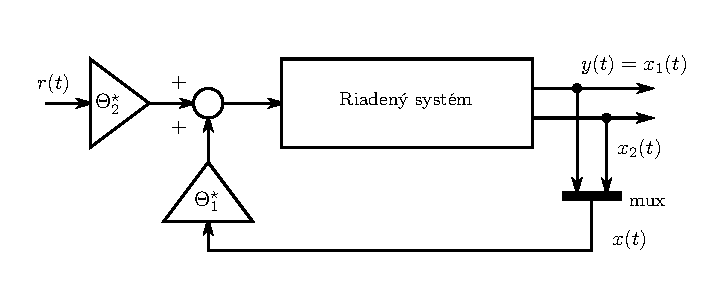
\includegraphics{Obr_41_ZRstavSpVaz_standalone.pdf}
    \caption{Zákon riadenia so stavovou spätnou väzbou -- pôvodný tvar, ktorý je umožnený pre dostupnosť stavového vektora $x(t)$.}
    \label{Obr_41_ZRstavSpVaz}
\end{figure}








Pre chybu pozorovania stavu $\tilde{x}_2(t)$ platí $\tilde{x}_2(t) = x_2(t) - \hat{x}_2(t)$. Dynamiku tejto chyby opisuje rovnica
\begin{equation}
	\dot{\tilde{x}}_2(t) = \left( A_{22} - L A_{12} \right) \tilde{x}_2(t)
\end{equation}
Z toho vyplýva, že vektor $L$ má byť zvolený tak, že matica $ A_{22} - L A_{12} $ je asymptoticky stabilná. Potom chyba pozorovania sa asymptoticky blíži k nule.

Získanie (meranie) signálu $\dot{x}_1(t)$ je z praktického hľadiska problematické. Preto sa zavádza signál $w(t)$ taký, že $\hat{x}_2(t) = w(t) + L y(t)$. Je zrejmé, že~$\dot{w}(t) = \dot{\hat{x}}_2(t) + L \dot{y}(t)$. Po dosadení a úpravách
\begin{equation}
	\dot{w}(t) =
	\left( A_{22} - L A_{12} \right) w(t)
	 +
	\left( A_{21} - L A_{11} + A_{22} L - L A_{12} L \right) y(t)
	 +
	\left( b_2 - L b_1 \right) u(t)
\end{equation}
S využitím $s$ ako operátora časovej derivácie je možné písať
\begin{equation}
	\begin{split}
		w(t)& =
			\left( sI - A_{22} + L A_{12} \right)^{-1}
			\left( A_{21} -  \right.   \left. - L A_{11} + A_{22} L - L A_{12} L \right) y(t)
						\\ & +
			\left( sI - A_{22} + L A_{12} \right)^{-1}
			\left( b_2 - L b_1 \right) u(t)
	\end{split}
\end{equation}
čo je možné vyjadriť aj v tvare
\begin{equation}
	w(t) =
	\text{diag}(g_u) \left[ \frac{\alpha(s)}{\Lambda(s)} \right] u(t)
	+
	\text{diag}(g_y) \left[ \frac{\alpha(s)}{\Lambda(s)} \right] y(t)
\end{equation}
kde $g_u \in \mathbb{R}^{n-1}$ a $g_y \in \mathbb{R}^{n-1}$ sú  vektory konštánt, preto $\text{diag}(g_u)$ a~$\text{diag}(g_y)$ sú diagonálne matice, $\alpha(s)$ je vektor mocnín operátora $s$ v tvare $\alpha^\naT(s) = \begin{bmatrix} s^{n-2}, \ldots,s, 1 \end{bmatrix}$ ak $n\geq 2$, inak $\alpha(s) = 0$, a nakoniec polynóm $\Lambda(s) = \text{det}\left( sI - A_{22} + L A_{12} \right)$ je monický Hurwitzov polynóm stupňa $n-1$ daný voľbou vektora $L$. Ako bolo uvedené $\hat{x}_2(t) = w(t) + L y(t)$, potom
\begin{equation}
	\hat{x}_2(t) =
	\text{diag}(g_u) \left[ \frac{\alpha(s)}{\Lambda(s)} \right] u(t)
	+
	\text{diag}(g_y) \left[ \frac{\alpha(s)}{\Lambda(s)} \right] y(t)
	+ L y(t)
\end{equation}





V úvode časti uvedený ideálny člen ${\Theta_1^\star}^\naT(t) x(t)$ je teda možné parametrizovať nasledovne. Stavový vektor $x(t)$ je nahradený odhadom $\hat{x}(t) = \begin{bmatrix} y(t) & \hat{x}_2(t) \end{bmatrix}^\naT$, a tiež sa rozdelí $\Theta_1^\star(t) = \begin{bmatrix} k_y^\star & {k_2^\star}^\naT \end{bmatrix}^\naT$, pričom $k_y^\star \in \mathbb{R}$, potom
\begin{equation} \label{n1param}
	\begin{split}
		{\Theta_1^\star}^\naT(t) \hat{x}(t)
		= &
		k_y^\star y(t) + {k_2^\star}^\naT \hat{x}_2(t)
		\\ = &
		k_y^\star y(t)
		+
		{k_2^\star}^\naT
		\text{diag}(g_u) \left[ \frac{\alpha(s)}{\Lambda(s)} \right] u(t)
		+
		{k_2^\star}^\naT
		\text{diag}(g_y) \left[ \frac{\alpha(s)}{\Lambda(s)} \right] y(t)
		+ {k_2^\star}^\naT L y(t)
	\end{split}
\end{equation}






\begin{figure}[t]
    \centering
    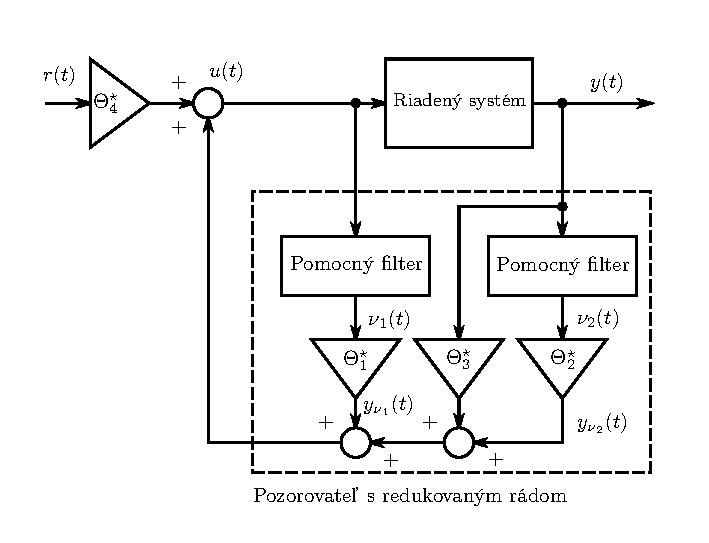
\includegraphics{Obr_PozRedRad_standalone.pdf}
    \caption{Pozorovateľ s redukovaným rádom.}
    \label{Obr_PozRedRad}
\end{figure}








V tomto bode text sa pre jednoduchosť a lepšiu názornosť zavedie úplne nové označovanie, ktorým sa mení označenie niektorých parametrov zákona riadenia, a teda význam pôvodného označovania. Pôvodný ideálny člen formálne zodpovedá výrazu ${\overline{\Theta}_1^\star}^\naT \hat{x}(t)$ a nové označovanie vyplýva zo zapísania rovnice \eqref{n1param} v tvare
\begin{equation} \label{n1param2}
	{\overline{\Theta}_1^\star}^\naT \hat{x}(t)
	=
	{\Theta_1^\star}^\naT \left[ \frac{\alpha(s)}{\Lambda(s)} \right] u(t)
	+
	{\Theta_2^\star}^\naT \left[ \frac{\alpha(s)}{\Lambda(s)} \right] y(t)
	+
	\Theta_3^\star y(t)
\end{equation}
kde sa vzhľadom na \eqref{n1param} zaviedlo označenie ${\Theta_1^\star}^\naT = {k_2^\star}^\naT \text{diag}(g_u)$,   ${\Theta_2^\star}^\naT = {k_2^\star}^\naT \text{diag}(g_y)$ a~$\Theta_3^\star = k_y^\star + {k_2^\star}^\naT L$.

Z uvedeného vyplýva, že ideálny stavový zákon riadenia použitý v predchádzajúcich častiach je možné re-parametrizovať do tvaru
\begin{equation} \label{n1reparamzr}
	u(t)
	=
	{\Theta_1^\star}^\naT \left[ \frac{\alpha(s)}{\Lambda(s)} \right] u(t)
	+
	{\Theta_2^\star}^\naT \left[ \frac{\alpha(s)}{\Lambda(s)} \right] y(t)
	+
	\Theta_3^\star y(t)
	+
	\Theta_4^\star r(t)
\end{equation}






V prvých dvoch členoch zákona riadenia \eqref{n1reparamzr} sú použité takzvané pomocné filtre. Tieto generujú pomocné signály $\nu_1(t)$ a $\nu_2(t)$ upresnené nižšie. Napríklad prvý člen pravej strany v rovnici \eqref{n1reparamzr} možno zapísať v tvare
\begin{equation}
	y_{\nu_1}(t) = {\Theta_1^\star}^\naT \left[\frac{\alpha(s)}{\Lambda(s)}\right] u(t)
	=
	\frac{
	\Theta_{1(n-2)}^\star s^{n-2}    + \cdots + \Theta_{11}^\star s + \Theta_{10}^\star
	}{
	s^{n-1}+ \lambda_{n-2} s^{n-2} + \cdots + \lambda_1 s + \lambda_0
	}
	u(t)
\end{equation}
kde $ \Theta_1^\star = \begin{bmatrix} \Theta_{1(n-2)}^\star  & \cdots & \Theta_{11}^\star & \Theta_{10}^\star \end{bmatrix}^\naT $, alebo v stavovom priestore v tvare \eqref{stavPriestPrvzPomFiltMRCp} na strane \pageref{stavPriestPrvzPomFiltMRCp}. Po označení jednotlivých vektorov a matíc v \eqref{stavPriestPrvzPomFiltMRCp} je prvý pomocný filter v~tvare
\begin{subequations}
	\begin{align}
		\dot \nu_1(t)
		&=
		\Lambda
		\nu_1(t)
		+
		q
		u(t)
		\\
		y_{\nu_1}(t)
		&=
		{\Theta_1^\star}^\naT
		\nu_1(t)
	\end{align}
\end{subequations}



Z uvedeného plynie, že prvý pomocný filter má v~stavovom priestore tvar $ \dot \nu_1(t) = \Lambda \nu_1(t) + q u(t) $, kde $\nu_1$(t) je vektor pomocných signálov generovaných prvým pomocným filtrom (stavový vektor prvého pomocného filtra). Tento je násobený parametrami zákona riadenia ${\Theta_1^\star}^\naT$. Analogicky, druhý prídavný filter má v stavovom priestore tvar $ \dot{\nu}_2(t) = \Lambda \nu_2(t) + q y(t) $. Zákon riadenia využívajúci len vstupno-výstupné signály riadeného systému je potom v tvare
\begin{align} \label{zakriadspoz}
	u(t) = {\Theta_1^\star}^\naT \nu_1(t) + {\Theta_2^\star}^\naT \nu_2(t) + \Theta_3^\star y(t) + \Theta_4^\star r(t)
\end{align}












\section{Formulácia problému riadenia s referenčným modelom}
\label{MRC problém}



Riešením MRC (Model Reference Control -- Riadenie s~referenčným modelom) problému je taký zákon riadenia $u$, ktorý zabezpečí, že výstup sústavy $y$~sleduje výstup referenčného modelu $y_m$~pri danom referenčnom signály $r$.



Uvažujme sústavu opísanú prenosovou funkciou v~tvare
\begin{equation} \label{PFsustavy_MRCp}
	\frac{y(s)}{u(s)} = k_p \frac{Z_p(s)}{R_p(s)}
\end{equation}
kde $Z_p(s)$ je monický, hurwitzov polynóm stupňa $m$, $R_p(s)$ je monický polynóm stupňa $n$ a~$k_p$~je tzv. \emph{vysokofrekvenčné zosilnenie sústavy}. \emph{Relatívny stupeň} sústavy je $n^* = n - m$.

Polynóm sa nazýva \emph{monický} ak je koeficient pri najvyššej mocnine $s$ (v~tomto prípade) rovný jednotke. Polynóm sa nazýva \emph{hurwitzov} ak sú reálne časti všetkých koreňov polynómu záporné.

Nech referenčný model je daný prenosovou funkciou v tvare
\begin{equation} \label{RefModelMRCp}
	\frac{y_m(s)}{r(s)} = W_m(s) = k_m \frac{Z_m(s)}{R_m(s)}
\end{equation}
kde $k_m$ je vysokofrekvenčné zosilnenie referenčného modelu, polynóm $Z_m(s)$ je monický Hurwitzov polynóm stupňa $m_m$, $R_m(s)$ monický Hurwitzov polynóm stupňa $n_m$, pričom relatívny stupeň $n^*_m = n_m - m_m = n^*$.

Zákon riadenia, ktorý rieši MRC problém je nasledovný. Najskôr uvedieme jeho všeobecný zápis, avšak pre lepšiu názornosť budeme riešenie MRC problému vyšetrovať na zjednodušenom konkrétnom príklade. Všeobecný tvar zákona riadenia, ktorý rieši MRC problém je
\begin{equation} \label{generalControlLaw}
    u = {\Theta_1^\star}^\naT \frac{\alpha(s)}{\Lambda(s)} u + {\Theta_2^\star}^\naT \frac{\alpha(s)}{\Lambda(s)} y + \Theta_3^\star y + \Theta_4^\star r
\end{equation}
kde $\alpha(s)$ je vektor obsahujúci mocniny $s$, $\alpha(s) = \begin{bmatrix} s^{n-2}, \ldots,s, 1 \end{bmatrix}^\naT$ ak $n\geq 2$, inak $\alpha(s) = 0$. Vektory $\Theta_1^\star \in \mathbb{R}^{n-1}$, $\Theta_2^\star \in \mathbb{R}^{n-1}$ a skaláry $\Theta_3^\star \in \mathbb{R}^1$, $\Theta_4^\star \in \mathbb{R}^1$ sú konštantné parametre zákona riadenia, ktorých hodnoty hľadáme.  $\Lambda(s)$ je ľubovolný monický Hurwitzov polynóm stupňa $n-1$ obsahujúci $Z_m(s)$ ako faktor
\begin{equation}
	\Lambda(s) = \Lambda_0(s) Z_m(s)
\end{equation}
a teda aj $\Lambda_0(s)$ je ľubovolný monický Hurwitzov polynóm zodpovedajúceho stupňa.








\subsection{Príklad pre systém 2. rádu}
\label{MRCproblemPriklad}



Uvažujme systém opísaný prenosovou funkciou v tvare
\begin{equation} \label{genaralFormOfPlant04}
	y(s) = k_p \frac{s + b_0}{ s^2 + a_1 s + a_0} \, u(s)
\end{equation}
kde $a_i, b_i$ sú konštanty ($b_0 > 0$). Referenčný model zvoľme tak aby mal rovnaký relatívny stupeň ako sústava.
\begin{equation}
	y_m(s) = W_m(s)r(s) = k_m \frac{s + b_{0m}}{ s^2 + a_{1m} s + a_{0m}} r(s)
\end{equation}

V tomto konkrétnom príklade, zákon riadenia, ktorý rieši MRC problém je v tvare
\begin{equation} \label{controlLaw}
	u(s) = \Theta_1^\star \frac{1}{(s + \lambda)} u(s) + \Theta_2^\star \frac{1}{(s + \lambda)} y(s) + \Theta_3^\star y(s) + \Theta_4^\star r(s)
\end{equation}
kde sme použili $\alpha(s) = 1$ a $\Lambda(s) = (s + \lambda)$. V tomto prípade $\Theta_1^\star$, $\Theta_2^\star$ aj $\Theta_3^\star$ a $\Theta_4^\star$ sú skalárne konštanty -- parametre zákona riadenia.
Zákon riadenia \eqref{controlLaw} možno upraviť do tvaru
\begin{subequations}
	\begin{align}
		\left( 1 - \frac{ \Theta_1^\star }{ (s + \lambda)} \right) u(s)
		&=
		\left( \frac{ \Theta_2^\star }{ (s + \lambda)} + \Theta_3^\star \right) y(s) + \Theta_4^\star r(s)
		\\
        \left( \frac{ (s + \lambda) - \Theta_1^\star }{ (s + \lambda)} \right) u(s)
		& =
		\left( \frac{ \Theta_2^\star + \Theta_3^\star (s + \lambda) }{ (s + \lambda)} \right) y(s) + \Theta_4^\star r(s)
		\\
		\label{controlLaw04_2}
		u(s) &= \frac{\Theta_2^\star + \Theta_3^\star (s + \lambda)}{(s + \lambda) - \Theta_1^\star} y(s) + \frac{ \Theta_4^\star (s + \lambda)}{(s + \lambda) - \Theta_1^\star} r(s)
	\end{align}
\end{subequations}






Dosadením \eqref{controlLaw04_2} do \eqref{genaralFormOfPlant04} získame prenosovú funkciu URO v tvare \eqref{MRCRovniceNavrchuStrany}:
\begin{subequations} \label{MRCRovniceNavrchuStrany}
	\begin{align}
		\begin{split}
		\label{genaralFormOfCL}
			y(s)
			=
			k_p
			\frac{
				s + b_0
				}{
				s^2 + a_1 s + a_0}
			\,
			\left(
				\frac{
					\Theta_2^\star
					+
					\Theta_3^\star
					(s + \lambda)
					}{
					(s + \lambda)
					-
					\Theta_1^\star}
				y(s)
				+
				\frac{
					\Theta_4^\star
					(s + \lambda)
					}{
					(s + \lambda)
					-
					\Theta_1^\star}
				r(s)
			\right)
		\end{split}
		\\
		\begin{split}
		\left(
			1
			-
			\frac{
				k_p
				(s + b_0)
				\left(
					\Theta_2^\star
					+
					\Theta_3^\star
					(s + \lambda)
				\right)
				}{
				(s^2 + a_1 s + a_0)
				\left(
					(s + \lambda)
					-
					\Theta_1^\star
				\right)}
		\right)
			y(s)
			=
			\frac{
				k_p
				(s + b_0)
				\Theta_4^\star
				(s + \lambda)
				}{
				(s^2 + a_1 s + a_0)
				\left(
					(s + \lambda)
					-
					\Theta_1^\star
				\right)}
			r(s)
		\end{split}
		\\
		\begin{split}
		\left(
			\frac{
				(s^2 + a_1 s + a_0)
				\left(
					(s + \lambda)
					-
					\Theta_1^\star
				\right)
				-
				k_p
				(s + b_0)
				\left(
					\Theta_2^\star
					+
					\Theta_3^\star
					(s + \lambda)
				\right)
				}{
				(s^2 + a_1 s + a_0)
				\left(
					(s + \lambda)
					-
					\Theta_1^\star
				\right)}
		\right)
			y(s)
			=\\=
			\frac{
				k_p
				(s + b_0)
				\Theta_4^\star
				(s + \lambda)
				}{
				(s^2 + a_1 s + a_0)
				\left(
					(s + \lambda)
					-
					\Theta_1^\star
				\right)}
				r(s)
		\end{split}
		\\
		\label{genaralFormOfCL_04}
		\begin{split}
			\frac{y(s)}{r(s)}
			=
			\frac{
				k_p
				(s + b_0)
				\Theta_4^\star
				(s + \lambda)
				}{
				(s^2 + a_1 s + a_0)
				\left(
					(s + \lambda)
					-
					\Theta_1^\star
				\right)
				-
				k_p
				(s + b_0)
				\left(
					\Theta_2^\star
					+
					\Theta_3^\star
					(s + \lambda)
				\right)}
		\end{split}
	\end{align}
\end{subequations}









Prenosovú funkciu \eqref{genaralFormOfCL_04} označme $G_c(s)$. Výstupná veličina sústavy bude sledovať výstupnú veličinu referenčného modelu ak $G_c(s) = W_m(s)$. Táto podmienka bude splnená ak
\begin{align}
	\Theta_4^\star &= \frac{k_m}{k_p} \label{idealTheta4} \\
	(s + \lambda) &= \Lambda_0(s) (s + b_{0m}) = (s + b_{0m}) \label{lambda}
\end{align}
pričom \eqref{idealTheta4} je prvou podmienkou zhody, \eqref{lambda} je voľbou polynómu $\Lambda(s)$ stupňa $n-1$ kde v tomto prípade $\Lambda_0(s) = 1$ a teda $\lambda = b_{0m}$ a druhou podmienkou zhody je
\begin{equation} \label{matchingEquation}
    \begin{split}
    	&(s^2 + a_1 s + a_0)
    	\left( (s + \lambda) - \Theta_1^\star \right)
    	-
    	k_p
    	(s + b_0)
    	\left( \Theta_2^\star + \Theta_3^\star (s + \lambda) \right)
    	\\&=
    	(s + b_0)   ( s^2 + a_{1m} s + a_{0m})
    \end{split}
\end{equation}
Potom možno \eqref{genaralFormOfCL_04} zapísať v tvare
\begin{equation} \label{genaralFormOfCL_05}
	\frac{y(s)}{r(s)}
	=
	\frac{
		k_p
		(s + b_0)
		\frac{k_m}{k_p}
		(s + b_{0m})
		}{
		(s + b_0)
		( s^2 + a_{1m} s + a_{0m})}
	=
	\frac{
		k_m
		(s + b_{0m})
		}{
		( s^2 + a_{1m} s + a_{0m})}
	=
	W_m(s)
\end{equation}
V prenosovej funkcii \eqref{genaralFormOfCL_05} dochádza ku vzájomnému  vykráteniu sa polynómu $(s + b_0)$. Táto operácia je možná, pretože tieto polynómy majú korene v zápornej polrovice komplexnej roviny a teda sú stabilné (Hurwitzove). Taký je predpoklad pre $Z_p(s)$. Polynómy, ktoré nie sú Hurwitzove nemožno v prenosovej funkcii navzájom vykrátiť. Podmienku zhody \eqref{matchingEquation} je možné zapísať aj v maticovom tvare porovnaním koeficientov pri rovnakých mocninách na oboch stranách
\begin{equation} \label{idealParameters}
	\begin{bmatrix}
		-1 & 0 & -k_p \\
		-a_1 & -k_p & -(k_p b_{0m} + k_p b_0) \\
		-a_0 & -k_p b_0 & -k_p b_0 b_{0m}
	\end{bmatrix}
	\begin{bmatrix}
    	  \Theta_1^\star \\
		  \Theta_2^\star \\
		  \Theta_3^\star
 	\end{bmatrix}
	=
	\begin{bmatrix}
    	a_{1m} + b_0 - b_{0m} - a_1 \\
    	a_{0m} + b_0 a_{1m} - a_1 b_{0m} - a_0 \\
    	b_0 a_{0m} - a_0 b_{0m}
  	\end{bmatrix}
\end{equation}
čo je sústava algebraických rovníc v tvare $M_s \Theta_s = p_s$ a~teda existencia takého vektora $\Theta_s$, ktorý spĺňa rovnosť, je závislá od vlastností matice $M_s$. Z~podmienok zhody \eqref{idealTheta4} a~\eqref{idealParameters} plynú konkrétne hodnoty parametrov zákona riadenia, ktoré riešia daný MRC problém.

Predchchádzajúci postup je možné zapísať prehladnejšie (pre prehľadnosť vynecháme aj zátvorky s laplaceovou premennou $(s)$):

Zákon riadenia
\begin{subequations}
	\begin{align}
		u
		&=
		\frac{\Theta_1^\star}{\Lambda}
		u
		+
		\frac{\Theta_2^\star}{\Lambda}
		y
		+
		\Theta_3^\star
		y
		+
		\Theta_4^\star
		r
		\\
		\left(
			1
			-
			\frac{\Theta_1^\star}{\Lambda}
		\right)
		u
		&=
		\left(
			\frac{\Theta_2^\star}{\Lambda}
			+
			\Theta_3^\star
		\right)
		y
		+
		\Theta_4^\star
		r
		\\
		\frac{\Lambda - \Theta_1^\star}{\Lambda}
		u
		&=
		\frac{
			\Theta_2^\star
			+
			\Theta_3^\star\Lambda
			}{
			\Lambda}
		y
		+
		\Theta_4^\star
		r
		\\
		u
		&=
		\frac{
			\Theta_2^\star
			+
			\Theta_3^\star\Lambda
			}{
			\Lambda - \Theta_1^\star}
		y
		+
		\frac{
		\Theta_4^\star \Lambda
		}{
		\Lambda - \Theta_1^\star}
		r
	\end{align}
\end{subequations}

Uzavretý regulačný obvod
\begin{subequations}
	\begin{align}
		y
		&=
		k_p
		\frac{Z_p}{R_p}
		\left(
				\frac{
			\Theta_2^\star
			+
			\Theta_3^\star\Lambda
			}{
			\Lambda - \Theta_1^\star}
		y
		+
		\frac{
		\Theta_4^\star \Lambda
		}{
		\Lambda - \Theta_1^\star}
		r
		\right)
\\
		\left(
			1
			-
			\frac{
				k_p
				Z_p
				\left(
					\Theta_2^\star
					+
					\Theta_3^\star\Lambda
				\right)
				}{
				R_p
				\left(
					\Lambda - \Theta_1^\star
				\right)}
		\right)
		y
		&=
		\frac{
			k_p
			Z_p
			\Theta_4^\star
			\Lambda
			}{
			R_p
			\left(
				\Lambda - \Theta_1^\star
			\right)}
		r
\\
		\frac{
			R_p
			\left(
				\Lambda - \Theta_1^\star
			\right)
			-
			k_p
			Z_p
			\left(
				\Theta_2^\star
				+
				\Theta_3^\star\Lambda
			\right)
			}{
			R_p
			\left(
				\Lambda - \Theta_1^\star
			\right)}
		y
		&=
		\frac{
			k_p
			Z_p
			\Theta_4^\star
			\Lambda
			}{
			R_p
			\left(
				\Lambda - \Theta_1^\star
			\right)}
		r
\\
		y
		&=
		\frac{
			k_p
			Z_p
			\Theta_4^\star
			\Lambda
			}{
			R_p
			\left(
				\Lambda - \Theta_1^\star
			\right)
			-
			k_p
			Z_p
			\left(
				\Theta_2^\star
				+
				\Theta_3^\star\Lambda
			\right)}
		r
	\end{align}
\end{subequations}

Podmienky zhody
\begin{subequations}
	\begin{align}
		\Theta_4^\star &= \frac{k_m}{k_p} \label{idealTheta4_02} \\
		\Lambda &= Z_m  \label{lambda_02}\\
		R_p \left( \Lambda - \Theta_1^\star \right) - k_p Z_p \left( \Theta_2^\star + \Theta_3^\star\Lambda \right)
		&=
		Z_p R_m
	\end{align}
\end{subequations}









\subsection{Zovšeobecnenie pre systém $n$. rádu}


Pri uvažovaní všeobecného zákona riadena v tvare \eqref{generalControlLaw} má prenosová funkcia uzavretého regulačného obvodu tvar
\begin{equation}
	y
	=
	\frac{
		k_p
		Z_p
		\Theta_4^\star
		\Lambda^2
		}{
		\Lambda
		\left(
			R_p
			\left(
				\Lambda - {\Theta_1^\star}^\naT	\alpha(s)
			\right)
			-
			k_p
			Z_p
			\left(
				{\Theta_2^\star}^\naT	\alpha(s)
				+
				\Theta_3^\star \Lambda
			\right)
		\right)}
	r
\end{equation}
a podmienky zhody
\begin{subequations}
	\begin{align}
		\Theta_4^\star &= \frac{k_m}{k_p} \label{idealTheta4_03} \\
		\Lambda &= \Lambda_0 Z_m \label{lambda_03} \\
		R_p
		\left(
			\Lambda - {\Theta_1^\star}^\naT \alpha(s)
		\right)
		-
		k_p
		Z_p
		\left(
			{\Theta_2^\star}^\naT \alpha(s)
			+
			\Theta_3^\star \Lambda
		\right)
	    &=
	    Z_p
	    \Lambda_0
	    R_m
	\end{align}
\end{subequations}

Predpoklady pri, ktorých sú tieto podmienky splniteľné sú intuitívne zrejmé z~predchádzajúceho príkladu v časti \ref{MRCproblemPriklad}. Hlbšou analýzou MRC problému sa v tomto kurze zaoberať nebudeme. Poslucháča odkazujeme na odporúčanú literatúru, kde nájde všetky potrebné (matematické) detaily k riešeniu MRC problému.









\section{Opis URO v stavovom priestore}

\subsection{Príklad pre systém 2. rádu}

V tejto časti vyjadríme uzavretý regulačný obvod, ktorý vznikne riešením MRC problému, pomocou opisu v~stavovom priestore. Opäť začneme zjednodušeným príkladom \ref{MRCproblemPriklad}, a~v~ďalšej časti dodáme pre úplnosť všeobecný zápis URO v~stavovom priestore.

Sústava v tvare \eqref{PFsustavy_MRCp}, konkrétne \eqref{genaralFormOfPlant04}, môže byť reprezentovaná opisom v~stavovom priestore v tvare
\begin{subequations}
	\begin{align}
		 \dot x &= A x + b u \\
		 y &= c^\naT x
	\end{align}
\end{subequations}
kde $x$ je vektor stavových veličín sústavy a $A$; $b$; $c^\naT$ sú konštantné matice (vektory) zodpovedajúcich rozmerov. V tomto prípade nekladieme žiadne podmienky na formu (kanonickú) matice $A$, ako to bolo v prípade stavového MRAC-u.

Uvažujeme zákon riadenia \eqref{controlLaw}, pripomeňme:
\begin{equation} \label{ZakonRiadeniaMRCp}
	u(s) = \Theta_1^\star \frac{1}{(s + \lambda)} u(s) + \Theta_2^\star \frac{1}{(s + \lambda)} y(s) + \Theta_3^\star y(s) + \Theta_4^\star r(s)
\end{equation}
V prvých dvoch členoch zákona riadenia \eqref{ZakonRiadeniaMRCp} sú použité takzvané prídavné filtre, ktorých vstupom je buď akčný zásah $u$ (vstupný signál sústavy) alebo výstupná (riadená) veličina $y$. Tieto prídavné filtre sú tiež nazývané pomocné, či prídavné generátory, generujú prídavné (pomocné) signály. Oba prídavné filtre sú rovnaké, v~ tomto prípade dané prenosovou funkciou $\frac{1}{(s + \lambda)}$. Výstupné signály filtrov sú v~tomto prípade skalárne signály. Vo všeobecnosti sú výstupné signály pomocných filtrov vektory signálov s~rovnakým rozmerom ako vektory parametrov $\Theta_1^\star$ a~$\Theta_2^\star$, viď všeobecný zápis zákona riadenia \eqref{generalControlLaw}. Označme výstupné signály prídavných filtrov $\nu_1$ a~$\nu_2$. Tieto signály sa násobia parametrami zákona riadenia ${{\Theta}_1^\star}$ a ${{\Theta}_2^\star}$. Prídané filtre možno zapísať v tvare
\begin{subequations}
	\begin{align}
		 \dot \nu_1 &= -\lambda \nu_1 + u \\
		 \dot \nu_2 &= -\lambda \nu_2 + y = -\lambda \nu_2 + c^\naT x
	\end{align}
\end{subequations}

Jednoduchým pridaním týchto pomocných signálov k sústave máme sústavu rovníc:
\begin{subequations} \label{DoplnenaSustavaMRCp}
	\begin{align}
		 \dot x &= A x + b u \\
		 \dot \nu_1 &= -\lambda \nu_1 + u \\
		 \dot \nu_2 &= -\lambda \nu_2 + c^\naT x \\
		 y &= c^\naT x
	\end{align}
\end{subequations}
Sústavu rovníc \eqref{DoplnenaSustavaMRCp} budeme nazývať \emph{doplnená sústava}. Doplnenú sústavu \eqref{DoplnenaSustavaMRCp} možno zapísať v maticovom tvare
\begin{subequations}
	\begin{align}
		\begin{bmatrix} \dot x \\ \dot{\nu}_1 \\ \dot{\nu}_2 \end{bmatrix}
		&=
		\begin{bmatrix} A & 0 & 0 \\ 0 & -\lambda & 0 \\ c^\naT & 0 & -\lambda \end{bmatrix}
	 	\begin{bmatrix} x \\ \nu_1 \\ \nu_2 \end{bmatrix}
		+
		\begin{bmatrix} b \\ 1\\ 0 \end{bmatrix}
	 	u
	 	\\
	 	y &= \begin{bmatrix} c^\naT & 0 & 0 \end{bmatrix}
	 	\begin{bmatrix} x \\ \nu_1 \\ \nu_2 \end{bmatrix}
	\end{align}
\end{subequations}
a po označení jednotlivých matíc a vektorov
\begin{subequations}
\label{augmentedPlant}
	\begin{align}
		 \dot X &= A_o X + B_c u \\
		 y &= C_c^\naT X \label{outputOfAugmentedPlant}
	\end{align}
\end{subequations}

Zákon riadenia \eqref{ZakonRiadeniaMRCp} zapíšeme v takom vektorovom tvare, v ktorom je možné využiť stavový vektor doplnenej sústavy $X$:
\begin{equation} \label{ZakonRiadeniaMaticMRCp}
	u = {\Theta_c^\star}^\naT D X + \Theta_4^\star r
\end{equation}
kde $ \Theta_c^\star = \begin{bmatrix} \Theta_3^\star & \Theta_1^\star & \Theta_2^\star \end{bmatrix}^\naT $; $\Theta_4^\star$ sú parametre zákona riadenia a maticu
\begin{align*}
	D = \begin{bmatrix} c^\naT & 0 & 0 \\ 0 & 1 & 0 \\ 0 & 0 & 1 \end{bmatrix}
\end{align*}
sme zaviedli práve preto aby sme v zákone riadenia \eqref{ZakonRiadeniaMaticMRCp} mohli priamo písať stavový vektor $X$. Tvar, v ktorom sa zákon riadenia \eqref{ZakonRiadeniaMaticMRCp} viac podobá na pôvodný zápis \eqref{ZakonRiadeniaMRCp}, a ktorý vyplíva priamo z \eqref{ZakonRiadeniaMaticMRCp} je
\begin{subequations} \label{ZakonRiadeniaMaticMRCp_02}
	\begin{align}
		u &= \Theta_1^\star \nu_1 + \Theta_2^\star \nu_2 + \Theta_3^\star {c}^\naT x + \Theta_4^\star r \\
		u &= \Theta_1^\star \nu_1 + \Theta_2^\star \nu_2 + \Theta_3^\star y + \Theta_4^\star r
	\end{align}
\end{subequations}









Dosadením \eqref{ZakonRiadeniaMaticMRCp} do \eqref{augmentedPlant} získame opis URO v~stavovom priestore v tvare (výstupnú rovnicu vynechávame, pretože sa nemení)
\begin{subequations} \label{UROaugmentedPlant}
	\begin{align}
		\dot X &= A_o X + B_c \left( {\Theta_c^\star}^\naT D X + \Theta_4^\star r \right) \\
		\dot X &= A_o X + B_c {\Theta_c^\star}^\naT D X + B_c \Theta_4^\star r \\
		\dot X &= \left( A_o + B_c {\Theta_c^\star}^\naT D \right) X + B_c \Theta_4^\star r \\
		\dot X &= A_c X + B_c \Theta_4^\star r
	\end{align}
\end{subequations}
kde
\begin{equation}
	\begin{split}
		A_c &= A_o + B_c {\Theta_c^\star}^\naT D \\
		&=
		\begin{bmatrix} A & 0 & 0 \\ 0 & -\lambda & 0 \\ c^\naT & 0 & -\lambda \end{bmatrix}
	 	+
	 	\begin{bmatrix} b \\ 1\\ 0 \end{bmatrix}
	 	\begin{bmatrix} \Theta_3^\star & \Theta_1^\star & \Theta_2^\star \end{bmatrix}
		\begin{bmatrix} c^\naT & 0 & 0 \\ 0 & 1 & 0 \\ 0 & 0 & 1 \end{bmatrix}
		\\
		&=
		\begin{bmatrix} A & 0 & 0 \\ 0 & -\lambda & 0 \\ c^\naT & 0 & -\lambda \end{bmatrix}
	 	+
	 	\begin{bmatrix} b \Theta_3^\star & b \Theta_1^\star & b \Theta_2^\star \\ \Theta_3^\star & \Theta_1^\star & \Theta_2^\star \\ 0 & 0 & 0 \end{bmatrix}
		\begin{bmatrix} c^\naT  & 0 & 0 \\ 0 & 1 & 0 \\ 0 & 0 & 1 \end{bmatrix}
		\\
		&=
		\begin{bmatrix} A & 0 & 0 \\ 0 & -\lambda & 0 \\ c^\naT & 0 & -\lambda \end{bmatrix}
	 	+
	 	\begin{bmatrix} b \Theta_3^\star c^\naT & b \Theta_1^\star & b \Theta_2^\star \\ \Theta_3^\star c^\naT & \Theta_1^\star & \Theta_2^\star \\ 0 & 0 & 0 \end{bmatrix}
		\\
		& =
		\begin{bmatrix} A +  b \Theta_3^\star c^\naT & b \Theta_1^\star & b \Theta_2^\star \\ \Theta_3^\star c^\naT & -\lambda + \Theta_1^\star & \Theta_2^\star \\ c^\naT & 0 & -\lambda \end{bmatrix}
	\end{split}
\end{equation}

Pretože uzavretý regulačný obvod zapísaný v tvare
\begin{subequations} \label{UROaugmentedPlant_02}
	\begin{align}
		\dot X &= A_c X + B_c \Theta_4^\star r \\
		y &= C_c^\naT X
	\end{align}
\end{subequations}
obsahuje ideálne parametre zákona riadenia, teda také, ktoré spĺňajú podmienky zhody musí sa tento zhodovať s referenčným modelom. Preto tzv. \emph{neminimálna reprezentácia} prenosovej funkcie referenčného modelu \eqref{RefModelMRCp} v stavovom priestore je
\begin{subequations} \label{NeminimalRMMRCp}
	\begin{align}
		\dot X_m &= A_c X_m + B_c \Theta_4^\star r \\
		y_m &= C_c^\naT X_m
	\end{align}
\end{subequations}
kde $X_m$ sú stavové veličiny neminimálnej reprezentácie modelu










\subsection{Systém $n$. rádu}




Uvažujeme zákon riadenia \eqref{generalControlLaw}, pripomeňme:
\begin{equation} \label{generalControlLaw_02}
	u = {\Theta_1^\star}^\naT \frac{\alpha(s)}{\Lambda(s)} u + {\Theta_2^\star}^\naT \frac{\alpha(s)}{\Lambda(s)} y + \Theta_3^\star y + \Theta_4^\star r
\end{equation}
kde $\alpha(s)$ je vektor obsahujúci mocniny $s$, $\alpha(s) = \begin{bmatrix} s^{n-2}, \ldots, s, 1 \end{bmatrix}^\naT$ ak $n\geq 2$, inak $\alpha(s) = 0$. Vektory ${\Theta_1^\star}, \Theta_2^\star \in \mathbb{R}^{n-1}$ a skaláry $\Theta_3^\star, \Theta_4^\star \in \mathbb{R}^1$ sú konštantné parametre zákona riadenia. $\Lambda(s)$ je ľubovolný monický Hurwitzov polynóm stupňa $n-1$.

Napríklad prvý člen v \eqref{generalControlLaw_02} možno zapísať v tvare
\begin{equation}
	y_{\nu_1} = {\Theta_1^\star}^\naT \frac{\alpha(s)}{\Lambda(s)} u
    =
	\frac{
	\Theta_{1(n-2)}^\star s^{n-2}    + \cdots + \Theta_{11}^\star s + \Theta_{10}^\star
	}{
	s^{n-1}+ \lambda_{n-2} s^{n-2} + \cdots + \lambda_1 s + \lambda_0
	}
	u
\end{equation}
kde $ \Theta_1^\star = \begin{bmatrix} \Theta_{1(n-2)}^\star  & \cdots & \Theta_{11}^\star & \Theta_{10}^\star \end{bmatrix}^\naT $, alebo v stavovom priestore v tvare
\begin{subequations} \label{stavPriestPrvzPomFiltMRCp}
	\begin{align}
		\begin{bmatrix}
			\dot{\nu}_{1(n-2)} \\
			\dot{\nu}_{1(n-3)} \\
			\dot{\nu}_{1(n-4)} \\
			\vdots \\
			\dot{\nu}_{10}
		\end{bmatrix}
		&=
		\begin{bmatrix}
			-\lambda_{n-2} & -\lambda_{n-3} &  \cdots & -\lambda_2 & -\lambda_1 & -\lambda_0\\
			1 & 0 &  \cdots & 0 & 0 & 0  \\
			0 & 1 & \ddots & 0 & 0 & 0 \\
			\vdots & \ddots & \ddots & \ddots & \vdots & \vdots \\
			0 & 0 & \ddots & 1 &  0 & 0 \\
			0 & 0 & \cdots & 0 &  1 & 0
		\end{bmatrix}
		\begin{bmatrix}
			\nu_{1(n-2)} \\
			\nu_{1(n-3)} \\
			\nu_{1(n-4)} \\
			\vdots \\
			\nu_{10}
		\end{bmatrix}
		+
		\begin{bmatrix}
			1 \\
			0 \\
			0 \\
			\vdots \\
			0
		\end{bmatrix}
		u
		\\
		y_{\nu_1}
		&=
		\begin{bmatrix}
			\Theta_{1(n-2)}^\star  &
			\Theta_{1(n-3)}^\star  &
			\Theta_{1(n-4)}^\star  &
			\cdots &
			\Theta_{10}^\star
		\end{bmatrix}
		\begin{bmatrix}
			\nu_{1(n-2)} \\
			\nu_{1(n-3)} \\
			\nu_{1(n-4)} \\
			\vdots \\
			\nu_{10}
		\end{bmatrix}
	\end{align}
\end{subequations}
Označme v \eqref{stavPriestPrvzPomFiltMRCp} jednotlivé vektory a maticu:
\begin{subequations}
	\begin{align}
		\dot \nu_1 &= \Lambda \nu_1 + q u \\
		y_{\nu_1} &= {\Theta_1^\star}^\naT \nu_1
	\end{align}
\end{subequations}



Z uvedeného vyplýva, že prvý prídavný filter má v~stavovom priestore tvar $\dot \nu_1 = \Lambda \nu_1 + q u $ kde $\nu_1$ je vektor pomocných signálov generovaných prvým pomocným generátorom (stavový vektor prvého pomocného generátora). Tento je násobený parametrami zákona riadenia ${\Theta_1^\star}^\naT$. Analogicky, druhý prídavný filter má v stavovom priestore tvar $\dot \nu_2 = \Lambda \nu_2 + q y = \Lambda \nu_2 + q c^\naT x$.
Doplnená sústava vo všeobecnom tvare je
\begin{subequations} \label{vsDoplnenaSustavaMRCp}
	\begin{align}
		\dot x &= A x + b u \\
		\dot \nu_1 &= \Lambda \nu_1 + q u \\
		\dot \nu_2 &= \Lambda \nu_2 + q c^\naT x \\
		 y &= c^\naT x
	\end{align}
\end{subequations}
Potom v \eqref{augmentedPlant} sú
\begin{align} \label{vsMaticeDoplnenejSustMRCp}
 	x = \begin{bmatrix} x \\ \nu_1 \\ \nu_2 \end{bmatrix}   ; \quad
	A_0 = \begin{bmatrix} A & 0 & 0 \\ 0 & \Lambda & 0 \\ q c^\naT & 0 & \Lambda \end{bmatrix}   ; \quad
	b_c = \begin{bmatrix} b \\ q\\ 0 \end{bmatrix}   ; \quad
    c_c^\naT = \begin{bmatrix} c^\naT & 0 & 0 \end{bmatrix}
\end{align}

Zákon riadenia \eqref{generalControlLaw_02} zapíšeme vo vektorovom tvare:
\begin{equation} \label{vsZakonRiadeniaMaticMRCp}
	u = {\Theta_c^\star}^\naT D x + \Theta_4^\star r
\end{equation}
kde $ \Theta_c^\star = \begin{bmatrix} \Theta_3^\star & {\Theta_1^\star}^\naT & {\Theta_2^\star}^\naT \end{bmatrix}^\naT; \; \Theta_4^\star $ sú parametre zákona riadenia a maticu
\begin{align*}
	D = \begin{bmatrix} c^\naT & 0 & 0 \\ 0 & I & 0 \\ 0 & 0 & I \end{bmatrix}
\end{align*}
sme zaviedli práve preto aby sme v zákone riadenia \eqref{vsZakonRiadeniaMaticMRCp} mohli priamo písať stavový vektor $x$. Tvar, v ktorom sa zákon riadenia \eqref{vsZakonRiadeniaMaticMRCp} viac podobá na pôvodný zápis \eqref{generalControlLaw_02}, a ktorý vyplíva priamo z \eqref{vsZakonRiadeniaMaticMRCp} je
\begin{subequations} \label{vsZakonRiadeniaMaticMRCp_02}
	\begin{align}
		u &= {\Theta_1^\star}^\naT \nu_1 + {\Theta_2^\star}^\naT \nu_2 + \Theta_3^\star {c}^\naT x + \Theta_4^\star r \\
		u &= {\Theta_1^\star}^\naT \nu_1 + {\Theta_2^\star}^\naT \nu_2 + \Theta_3^\star y + \Theta_4^\star r
	\end{align}
\end{subequations}

Dosadením \eqref{vsZakonRiadeniaMaticMRCp} do \eqref{augmentedPlant}, v ktorej sú ale matice \eqref{vsMaticeDoplnenejSustMRCp}, získame opis URO v~stavovom priestore v tvare \eqref{UROaugmentedPlant_02}, a~matica
 $A_c$  má tvar
\begin{equation}
	\begin{split}
		A_c &= A_o + b_c {\Theta_c^\star}^\naT D \\
		&=
        \begin{bmatrix}  A & 0 & 0 \\ 0 & \Lambda & 0 \\ q c^\naT & 0 & \Lambda \end{bmatrix}
	 	+
	 	\begin{bmatrix} b \\ q\\ 0 \end{bmatrix}
	 	\begin{bmatrix} \Theta_3^\star & {\Theta_1^\star}^\naT & {\Theta_2^\star}^\naT \end{bmatrix}
		\begin{bmatrix} c^\naT & 0 & 0 \\ 0 & I & 0 \\ 0 & 0 & I \end{bmatrix} \\
		&=
        \begin{bmatrix} A & 0 & 0 \\ 0 & \Lambda & 0 \\ q c^\naT & 0 & \Lambda \end{bmatrix}
	 	+
	 	\begin{bmatrix}
			b \Theta_3^\star & b {\Theta_1^\star}^\naT & b {\Theta_2^\star}^\naT \\
			q \Theta_3^\star & q {\Theta_1^\star}^\naT & q {\Theta_2^\star}^\naT \\
			0 & 0 & 0
		\end{bmatrix}
		\begin{bmatrix} c^\naT  & 0 & 0 \\ 0 & I & 0 \\ 0 & 0 & I \end{bmatrix} \\
		&=
		\begin{bmatrix} A & 0 & 0 \\ 0 & \Lambda & 0 \\ q c^\naT & 0 & \Lambda \end{bmatrix}
	 	+
	 	\begin{bmatrix}
			b \Theta_3^\star c^\naT & b {\Theta_1^\star}^\naT & b {\Theta_2^\star}^\naT \\
			q \Theta_3^\star c^\naT & q {\Theta_1^\star}^\naT & q {\Theta_2^\star}^\naT \\
			0 & 0 & 0
		\end{bmatrix} \\
		&=
		\begin{bmatrix}
             A +  b \Theta_3^\star c^\naT&
	    	 b {\Theta_1^\star}^\naT &
	    	 b {\Theta_2^\star}^\naT \\
	    	 q \Theta_3^\star c^\naT &
	    	 \Lambda + q {\Theta_1^\star}^\naT &
	    	 q {\Theta_2^\star}^\naT \\
	    	 q c^\naT & 0 & \Lambda
	 	\end{bmatrix}
	\end{split}
\end{equation}

Pretože takto všeobecne opísaný URO obsahuje ideálne parametre zákona riadenia, teda také, ktoré spĺňajú podmienky zhody musí sa tento zhodovať so všeobecným referenčným modelom \eqref{RefModelMRCp}, ktorého neminimálna reprezentácia v~stavovom priestore má tvar
\begin{subequations} \label{vsNeminimalRMMRCp}
	\begin{align}
		\dot x_m &= A_c x_m + \overline{b}_c r \\
		y_m &= c_c^\naT x_m
	\end{align}
\end{subequations}
kde $x_m$ sú stavové veličiny neminimálnej reprezentácie referenčného modelu a kde sme označili $\overline{b}_c = b_c \Theta_4^\star$.













\section{Cvičenie siedme}
\label{cvicsiedme}


\begin{enumerate}

    \item Uvažujme riadený systém\footnote{Uvedený riadený systém je prevzatý z článku publikovanom v prestížnom elektronickom časopise posterus.sk (nemýliť si so Slniečkom, už nevychádza), viď \cite{Tar11}.}, ktorý pracuje v pásme danom dvomi pracovnými bodmi. V~týchto dvoch hraničných pracovných bodoch prenosová funkcia systému nie je rovnaká, vyskytujú sa mierne rozdiely v~hodnotách koeficientov jednotlivých polynómov, pričom stupne polynómov sú zhodné, konkrétne:
    \begin{align}
    	G_{OP_1} &= 0,1659 \frac{s + 22}{ s^2 + 3,1423 s + 2,6539} 	\label{plantModel1}\\
    	G_{OP_2} &= 0,1669 \frac{s + 20,7618}{s^2 + 2,3422s + 2,7293} \label{plantModel2}
    \end{align}
    \begin{itemize}
    	\item Určte \emph{nominálnu} prenosovú funkciu sústavy tak, že jej koeficienty sú priemery hodnôt oboch prenosových funkcií \eqref{plantModel1} a~\eqref{plantModel2}.

    	\item Pre nominálnu prenosovú funkciu sústavy určte polynómy $Z_p$, $R_p$ a~zosilnenie $k_p$ pričom
    	\begin{equation} \label{C_PFsustavy_MRCp}
    	       \frac{y(s)}{u(s)} = k_p \frac{Z_p(s)}{R_p(s)}
        \end{equation}
        kde $Z_p(s)$ je monický  polynóm stupňa $m$, $R_p(s)$ je monický polynóm stupňa $n$ a~$k_p$ je tzv. \emph{vysokofrekvenčné zosilnenie sústavy}. \emph{Relatívny stupeň} sústavy je $n^* = n - m$.

        \item Zistite, či polynóm $Z_p(s)$ je Hurwitzov.
    \end{itemize}



    \item Vyriešte MRC problém pre nominálnu prenosovú funkciu sústavy, uvažujte referenčný model daný prenosovou funkciou v~tvare
    \begin{equation}
    	W_m(s) = \frac{s + 3}{ s^2 + 3.5 s + 3}
    \end{equation}
    Referenčný model je daný prenosovou funkciou v~tvare
    \begin{equation} \label{C_RefModelMRCp}
    	\frac{y_m(s)}{r(s)} = W_m(s) = k_m \frac{Z_m(s)}{R_m(s)}
    \end{equation}
    kde $k_m$ je vysokofrekvenčné zosilnenie referenčného modelu, $Z_m(s)$ monický Hurwitzov polynóm stupňa $m_m$, $R_m(s)$ monický Hurwitzov polynóm stupňa $n_m$, pričom relatívny stupeň $n^*_m = n_m - m_m = n^*$.

    Riešením MRC problému je taký zákon riadenia $u$, ktorý zabezpečí, že výstup sústavy $y$~sleduje výstup referenčného modelu $y_m$ pri danom referenčnom signály (vstupe referenčného modelu) $r$. Všeobecný tvar zákona riadenia, ktorý rieši MRC problém je
    \begin{equation} \label{C_generalControlLaw}
    	u = {\Theta_1^\star}^\naT \frac{\alpha(s)}{\Lambda(s)} u + {\Theta_2^\star}^\naT \frac{\alpha(s)}{\Lambda(s)} y + \Theta_3^\star y + \Theta_4^\star r
    \end{equation}
    kde $\alpha(s)$ je vektor obsahujúci mocniny $s$, $\alpha(s) = \begin{bmatrix} s^{n-2}, \ldots,s, 1 \end{bmatrix}^\naT$ ak $n\geq 2$, inak $\alpha(s) = 0$. Vektory $\Theta_1^\star \in \mathbb{R}^{n-1}$, $\Theta_2^\star \in \mathbb{R}^{n-1}$ a skaláry $\Theta_3^\star \in \mathbb{R}^1$, $\Theta_4^\star \in \mathbb{R}^1$ sú konštantné parametre zákona riadenia, ktorých hodnoty hľadáme.  $\Lambda(s)$ je ľubovolný monický Hurwitzov polynóm stupňa $n-1$ obsahujúci $Z_m(s)$ ako faktor
    \begin{equation}
    	\Lambda(s) = \Lambda_0(s) Z_m(s)
    \end{equation}
    a teda aj $\Lambda_0(s)$ je ľubovolný monický Hurwitzov polynóm zodpovedajúceho stupňa.


    \begin{itemize}
    	\item Na základe všeobecného tvaru zákona riadenia \eqref{C_generalControlLaw} určte zákon riadenia pre uvažovaný konkrétny prípad.
    	\item Vypočítajte parametre $\Theta_1^\star$, $\Theta_2^\star$, $\Theta_3^\star$, $\Theta_4^\star$.
    	\item Zostavte simulačnú schému uzavretého regulačného obvodu a overte vypočítané parametre zákona riadenia.
    \end{itemize}





\end{enumerate}















\section*{Otázky a úlohy}
\addcontentsline{toc}{section}{Otázky a úlohy}




\begin{enumerate}



    \item Je daný model systému
    \begin{align*}
        \dot{x}_1(t) &= x_2(t) \\
        \dot{x}_2(t) &= -a_1 x_2(t) - a_0 x_1(t) + b_0 u(t) \\
        y(t) & = x_1(t)
    \end{align*}
    kde $a_0, a_1, b_0 > 0$ sú neznáme parametre systému, $u(t)$ je vstup, $y(t)$ je výstup a~$x_1(t)$, $x_2(t)$ sú stavové veličiny systému. Tiež je daný referenčný model v tvare
    \begin{align*}
        \begin{bmatrix} \dot{x}_{1m}(t) \\ \dot{x}_{2m}(t) \end{bmatrix}
        &=
        \begin{bmatrix} 0 & 1 \\ -a_{0m} & -a_{1m} \end{bmatrix}
        \begin{bmatrix} x_{1m}(t)  \\ x_{2m}(t) \end{bmatrix}
        +
        \begin{bmatrix} 0  \\  b_{0m} \end{bmatrix}
        r(t) \\
        y_m(t) &= \begin{bmatrix} 1 & 0 \end{bmatrix}
        \begin{bmatrix} x_{1m}(t) \\ x_{2m}(t) \end{bmatrix}
    \end{align*}
    kde $a_{0m}, a_{1m}, b_{0m} > 0$ sú známe parametre referenčného modelu, $r(t)$ je referenčný signál, $y_m(t)$ je výstup a~$x_{1m}(t)$, $x_{2m}(t)$ sú stavové veličiny referenčného modelu.
    \begin{enumerate}
        \item Napíšte model systému v tvare prenosovej funkcie \label{odvodtePrenosFcn}
        \begin{equation*}
            \frac{y(s)}{u(s)} = k_p \frac{Z_p(s)}{R_p(s)}
        \end{equation*}
        kde $Z_p(s)$ je monický, hurwitzov polynóm stupňa $m$, $R_p(s)$ je monický polynóm stupňa $n$ a~$k_p$~je vysokofrekvenčné zosilnenie sústavy. Napíšte referenčný model v tvare prenosovej funkcie
        \begin{equation*}
            \frac{y_m(s)}{r(s)} = W_m(s) = k_m \frac{Z_m(s)}{R_m(s)}
        \end{equation*}
        kde $k_m$ je vysokofrekvenčné zosilnenie referenčného modelu, polynóm $Z_m(s)$ je monický Hurwitzov polynóm stupňa $m_m$, $R_m(s)$ monický Hurwitzov polynóm stupňa $n_m$.

        \item Cieľom riadenia je $y = y_m$. Navrhnite ideálny zákon riadenia v~tvare
        \begin{equation*}
            u = {\Theta_1^\star}^\naT \frac{\alpha(s)}{\Lambda(s)} u + {\Theta_2^\star}^\naT \frac{\alpha(s)}{\Lambda(s)} y + \Theta_3^\star y + \Theta_4^\star r
        \end{equation*}
        kde $\alpha(s)$ je vektor obsahujúci mocniny $s$, $\alpha(s) = \begin{bmatrix} s^{n-2}, \ldots,s, 1 \end{bmatrix}^{\mathsf{T}}$ ak $n\geq 2$, inak $\alpha(s) = 0$. Vektory $\Theta_1^\star, \Theta_2^\star \in \mathbb{R}^{n-1}$ a  skaláry $\Theta_3^\star, \Theta_4^\star \in \mathbb{R}^1$ sú konštantné parametre zákona riadenia, ktorých hodnoty hľadáme.  $\Lambda(s)$ je ľubovolný monický Hurwitzov polynóm stupňa $n-1$ obsahujúci $Z_m(s)$ ako faktor
        \begin{equation*}
            \Lambda(s) = \Lambda_0(s) Z_m(s)
        \end{equation*}
        a teda aj $\Lambda_0(s)$ je ľubovolný monický Hurwitzov polynóm zodpovedajúceho stupňa.
    \end{enumerate}



    \bigskip

    \item Odvoďte podmienky zhody pre MRAC vstupno-výstupný

    \medskip

    \item Odvoďte podmienky zhody uzavretého regulačného obvodu a referenčného modelu.

        \begin{tabular}{@{}l @{\ } l}
            Model riadeného systému: &
            $\displaystyle \frac{y(s)}{u(s)} = k_p\frac{Z_p(s)}{R_p(s)}$
            \qquad
            \begin{tabular}{@{}l}
            rád systému $n = 2$\\
            relatívny stupeň $n^* = 1$
            \end{tabular} \vspace{1mm}\\
            Referenčný model: & $\displaystyle \frac{y_m(s)}{r(s)} = k_m\frac{Z_m(s)}{R_m(s)} $ \vspace{1mm} \\
            Zákon riadenia: & $\displaystyle u(s) = \frac{\Theta_1^\star}{\Lambda(s)} u(s) + \frac{\Theta_2^\star}{\Lambda(s)} y(s) + \Theta_3^\star y(s) + \Theta_4^\star r(s)$
        \end{tabular}






\end{enumerate}




\bibliography{misc/Bib_KurzAR}{}
\bibliographystyle{plain}


















\end{document}
